% !TeX spellcheck = en_GB
\documentclass[../summary.tex]{subfiles}

\begin{document}
	
	\section{Global governance}
	
	\subsection{Study guide}
		\label{sec:13-study-guide}
	
	\begin{itemize}
		\item You should clearly understand the concepts discussed in the module and be able to recognize examples.
		\item Important concepts: principle of sustainable development, intergenerational equity, principle of sustainable use, intragenerational equity, integration principle, national
		sovereignty, principle of preventive action, precautionary principle, polluter pays principle, common but differentiated responsibility, risk assessment, environmental justice (with all its elements), collective action problem, multilateral negotiations, polycentric governance
	\end{itemize}
	
	You don’t need to read the court rulings on Bayer and chlorothalonil in chapter 3.3. The text 'Legal aspects of the choice of environmental policy instruments from the point of view of Belgian, European and international law' in chapter 4.1 does not have to be studied. You don’t need to memorize the conventions’ names or years in chapter 5.2.
	
	\subsection{Jurisdiction}
		\subsubsection{Legal principles of sustainable development}
			This part of the course introduces the principles of sustainable development based on the 1992 Rio Declaration and its updates.
			
			\paragraph{The principle of sustainable development}\mbox{}\\
				\label{par:13-princ-sus-dev}
				Principle three of the Rio Declaration states:
				\begin{quote}
					The right to development must be fulfilled so as to equitably meet developmental and environmental needs of present and future generations. 
				\end{quote}
				This principle originated from the World commission on Environment and Development, better known as the Brundtland Commission. It came as a response to address the accelerating deterioration of the environment. Because of the work done by this commission we have a definition of `sustainable development'. It takes the form of a three-tier concept encompassing ecological, social and economic development.\\
				\\
				In international law, sustainable development is mainly broken down into four parts:
				\begin{itemize}
					\item The principle of intergenerational equity, which amounts to the need to preserve resources for future generations. 
					\item The principle of sustainable use refers to a more immediate concern to use resources wisely.
					\item Intra-generational equity implies the balanced use of the world's resources by the various parts of the world
					\item The principle of integration implies that environmental considerations are taken into account in economic and development objectives. 
				\end{itemize}
				\newpage
				
			\paragraph{National sovereignty over natural resources}\mbox{}\\
				\label{par:national-sovereignty-over-natural-resources}
				Principle two of the Rio Declaration reads as follows:
				\begin{quote}
					States have, in accordance with the Charter of the United Nations and the principles of international law, the sovereign right to exploit their own resources pursuant to their own environmental and developmental policies, and the responsibility to ensure that activities within their jurisdiction or control do not cause damage to the environment of other States or of areas beyond the limits of national jurisdiction
				\end{quote}
				This essentially means that the international laws about sustainability have State sovereignty over its own resources as a cornerstone. However, this does not mean that States can do whatever they like, they can not inflict damage to the territory of other States for example. Environmental challenge the classic theory of international law regarding territory and State sovereignty.  This is why there is a relatively new part of a States sovereignty: the protection of the global commons. This was added to the traditional three regimes vis-à-vis jurisdiction:
				\begin{itemize}
					\item The majority of the Earth is subject to territorial sovereignty.
					\item Res nullius are those parts of the Earth which are capable of lawful national appropriation/sovereignty, but are as yet unclaimed.
					\item Res communis are shared by all nations and cannot be placed under State sovereignty
				\end{itemize}
				Especially the distinction between global commons and res communis is relevant. The largest challenge is to find a way for parties to adjudicate regulatory power over the global commons. There are some concerns about:
				\begin{itemize}
					\item Alleviates veto concerns: one can not assume that global consensus will be found over issues concerning global commons. If this was the case, every State would effectively hold veto power over the management of these. 
					\item Unbridled unilateralism or even selective multilateralism indeed would risk rewarding coercion.
				\end{itemize}
				
			\paragraph{The principle of preventive action and the precautionary principle}\mbox{}\\
				Principle two seen in paragraph \ref{par:national-sovereignty-over-natural-resources} in combination with principle 15 of the Rio Declaration define the prevention principle: 
				\begin{quote}
					In order to protect the environment, the precautionary approach shall be widely applied by States according to their capabilities. Where there are threats of serious or irreversible damage, lack of full scientific certainty shall not be used as a reason for postponing cost-effective measures to prevent environmental degradation
				\end{quote}
				This principle obliges authorities to take action at the earliest possible stage to prevent known risks from being realized. There however is not an undisputed definition of the precautionary principle. Generally though, it is defined in a more negative sense: States must not defer regulatory action even if there is no conclusive scientific proof between a given (in)action and damage to the human health or environment.\\
				\\
				As for the content of the principles, they can be distinguished in terms of the types of risks one has to manage. Preventative deals with known risk and precautionary deals with uncertain risks. The former is also part of international law while the latter is again disputed. 
				\newpage
				
			\paragraph{The polluter pays principle}\mbox{}\\
				Principle 16 of the Rio Declaration states:
				\begin{quote}
					National authorities should endeavour to promote the internalization of environmental costs and the use of economic instruments, taking into account the approach that the polluter should, in principle, bear the cost of pollution, with due regard to the public interest and without distorting international trade and investment
				\end{quote}
				The polluter pays principle requires all environmental costs to be internalized by the companies which cause them. Theoretically full introduction of this would result in this being a cost on a company's account. In reality the principle is faced with a lot of many challenges. For example, it is not easy to calculate the economic value of pollution. When this is feasible though, one still  needs to find the polluter and be able to hold them accountable.  The biggest obstacle by far is the unwillingness of politicians to actually implement this into the law.
				
			\paragraph{Common but differentiated responsibility}\mbox{}\\
				\label{par:13-comm-diff-res}
				Principle seven of the Rio Declaration states:
				\begin{quote}
					States shall cooperate in a spirit of global partnership to conserve, protect and restore the health and integrity of the Earth's ecosystem. In view of the different contributions to global environmental degradation, States have common but differentiated responsibilities. The developed countries acknowledge the responsibility that they bear in the international pursuit of sustainable development in view of the pressures their societies place on the global environment and of the technologies and financial resources they command
				\end{quote}
				This principle is one of common sense, although it can be quite sensitive at times. Because of the wording used to make this principles, countries like China and India think they have the right to postpone their climate efforts. 
				% Amai het is ook duidelijk dat de kindjes minder en minder goesting hadden naar mate dat ze verder geraakte met deze kut principals
				
			\subsubsection{Law enables and disables}
				The law can be used as a shield and as a sword. For example when someone steals your bike, you can use the receipt you got as a sword to prove that the bike is yours. On the other hand, if you are falsely accused of stealing that bike, you can use the same receipt as a shield to protect yourself and your bike. \\
				\\
				These concepts also apply to international law, however it is much more difficult to use the law as a sword because of the vague wording used to make these laws. In practise they are good shields for States to protect themselves but bad swords for parties who want to fight lacklustre attempts from States to follow these laws. 
				\newpage
				
	\subsection{Law and science}
		\subsubsection{Risk regulation: an introduction}
			\paragraph{Benzene and the risk assessment revolution}\mbox{}\\
				Benzene is an influential court case handled by the US Supreme Court. It is widely seen as having introduced risk assessment as the default standard for risk analysis by US regulators as it led to the commissioning of the National Research Council (NRC). \\
				\\
				The resulting risk assessment guidelines in the US Government hold 10 recommendations. It acknowledges that assessment can not be made completely free of policy considerations, but emphasized that steps should be taken to  manage and assess risks. The ultimate aim of these guidelines in dealing with risk is `to evaluate trade-offs between health consequences and other effects of specific regulatory actions.' 
				
			\paragraph{Risk assessment in the EU}\mbox{}\\
				The EU has only recently started to consider the conceptual approach to risk analysis as carried out at the EU level. Three main developments have led to the current approach to risk management. 
				
				\subparagraph{National risk management failures and their backlash at the EU level}\mbox{}\\
					Generally, regulatory failures often drive regulatory developments. Precious little regulatory law is inspired by a purely academic risk analysis exercise. Quite literally, from the ashes of disaster grow the roses (whether or not thorny) of regulatory success.
				
				\subparagraph{Governance and the impact on regulation}\mbox{}\\
					The European Commission has highlighted the increasing reliance, in the development of EU regulatory law, on expert advice, and the consequential need on public trust in that advice.
					
				\subparagraph{The impact of the precautionary principle}\mbox{}\\
					In 2000 the EU adopted a Communication on the precautionary principle which is arguably the highest-profile attempt to translate the principle into guidelines. The Commission insists in this document that the precautionary principle in its European context is a justified part of risk management.
					
				The EU and its Member States view risk analysis as a linear process, in which the various steps of a risk analysis process (risk identification, risk assessment, risk management, and risk communication), are neatly divided. Importantly, the EU assigns the responsibility and the main lead in each of these steps to different professional groupings. Whilst the steps of risk identification and certainly that of risk assessment are a responsibility of scientists, the step of risk management is very firmly seen as a political step, in which elected politicians on both the national scene and the European scene, take the lead. This preponderant role of politicians in risk management, makes the process prone, so its critics say, to being susceptible to scaremongering, and to recourse to the precautionary principle.
				
			\paragraph{The law is in awe of science}\mbox{}\\
				Many people believe that the law should be based on objective scientific facts. This has been the standard for global law when it comes to regulating risks, usually taking the form of risk analysis. We distinguish four steps during this process:
				\begin{description}
					\item[Risk Identification] The identification of a potential risk: `I wonder what the impact would be if ...'
					\item[Risk Assessment] This is the objective scientific step where we assess what happens, what impact there could be, what will it cost to solve this problem... 
					\item[Risk Management] What should we do about the risk that we have just explored in our scientific arguments? This step is also very different depending on which part of the world you are in, even though it is based on the same objective facts established in the previous step.
					\item[Risk Communication] Communicate the risk management measure that you have taken. 
				\end{description} 
				
	\subsection{Regulation vs. liability}
		\subsubsection{Types of regulation}
			As seen in the study guide (section \ref{sec:13-study-guide}), this is irrelevant for the exam.
		
		\subsubsection{How does a regulator regulate}
			To give an illustration from the real world, we look at \textbf{Article 191} of the Treaty on the Functioning of the European Union. This article instructs the European Commission (EC) on how to create policy for environmental protection. \textbf{The EC essentially has to take into account a `high level' of environmental protection}, because the article functions as the starting point for environmental policy. Even though this sounds good, the article immediately goes on to nuance its standpoint.\\
			\\
			 For example, they need to take into account \textbf{`available scientific and technical data'} to make a law, but in a lot of cases this is not present: for example, the effect of asbestos on people was not known when it was introduced.  Furthermore, the EC must take into account \textbf{`environmental conditions in the various regions of the Union'}, complicating matters even more. Thirdly, the EC as to take \textbf{`the potential benefits and costs of action or lack of action'} into account. This is not always easy because what is protecting the environment actually worth to us? Lastly, the EC needs to take into account \textbf{`the economic and social development of the union as a whole and the balanced development of its regions'}.
	
	\subsection{Environmental justice}
		\subsubsection{A history of environmental governance}
			Initially, environmental policy started at the national level of a State. Specifically in the US, the triggering event was the discovery of the hazards of DDT. Somewhere along the line, countries realized that pollution doesn't stop at the border. Since globalization has grown fast, countries increasingly consume products that were produced elsewhere.
			This means that people's consumption can cause environmental harm outside of their country. This external impact often is called an \textbf{external footprint}. \\
			\\
			For example, an external footprint is that 75\% of greenhouse gas emissions costs by producing the clothes, footwear and household textiles that we consume in the European Union, actually occurred outside of Europe. Another example is that EU consumption causes 10\% of global deforestation, almost all of which takes place outside the EU. Finally, EU food imports causes external land and water use impacts. These examples demonstrate how countries and the European Union bear responsibility for environmental problems outside their borders. \textbf{Those environmental problems can only be addressed through collaboration with other countries}.\\
			\\
			Against a backdrop of growing globalization and the transboundary nature of environmental pollution, many of the problems that we face are so-called \textbf{collective action problems}. They are characterized by a situation in which multiple individuals or countries would benefit from a certain action. But that action comes at a cost. Which is why individuals are unlikely to pay that cost if the others are not doing likewise. Costly decisions are thus made individually, but the benefits are for everyone. In such a situation, voluntary change seems unlikely. Some authoritative agreement or organization seems required to make everyone contribute to addressing the problem.\\
			\\
			In order to solve these problems together, a number of pioneering countries set the international political agenda, which led to the first global environmental conference. This gave rise to the United Nations Environment Program (UNEP) which monitors the global environment. Later, the Brundtland report discussed in paragraph \ref{par:13-princ-sus-dev} came out and gave rise to the Rio Declaration. \\
			\\
			Over the next 10 to 20 years, updates were made to declarations and proposals such as the Rio Declaration. This brought the issues at hand back into focus for political leaders. Finally, this led to the creation of the sustainable development goals or SDGs. 
		
		\subsubsection{Environmental justice}
			In 2019, \emph{the French} held the yellow vest protests against rising taxes for fossil fuels. This clearly showed that environmental policy should take social aspects into account. It is important to think about the effects of a policy change so that it does not disproportionally hit a certain group of the society. The film `Erin Brokovich' also illustrated these principals.\\
			\\
			To summarise, \textbf{environmental justice} is a \textbf{multifaceted concept that varies depending on issue, context and analysts}. Although the two examples are local ones, environmental justice \textbf{plays an important role from the local to the global level}. Essentially, we have to \textbf{ensure equity between privileged and unprivileged groups and individuals}. 
		
		% \subsubsection{Case: PFOS scandal in Flanders, Belgium}
		\stepcounter{subsubsection} % This line is purely to make the numbering seem right on the PDF
		
		\subsubsection{Elements of environmental justice}
			There are three main aspects or elements of environmental justice as depicted in figure \ref{fig:13-elements-of-justice}.
			\begin{description}
				\item[Distribution] How are costs and benefits allocated among actors? This is already included in the Rio Declaration discussed in paragraph \ref{par:13-comm-diff-res}.
				\item[Recognition] Are differences respected? Do certain actors dominate?
				\item[Procedure] How are decisions made and by whom? This is about an inclusive process and enabling every actor to participate.
			\end{description}
			\begin{figure}[h]
				\centering
				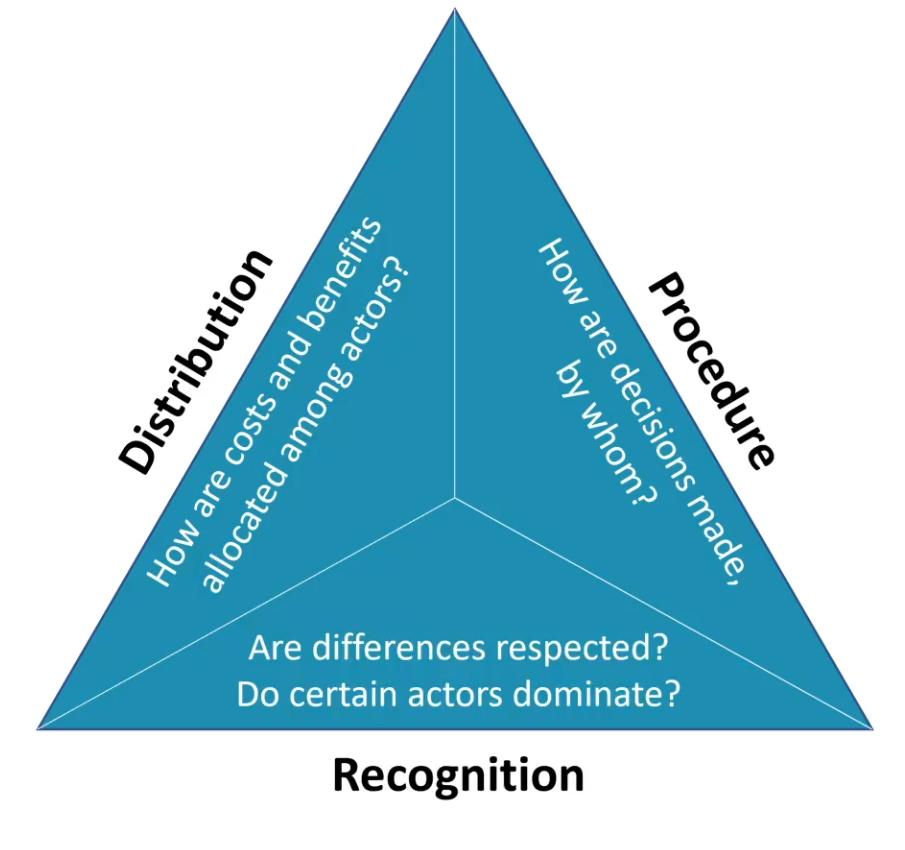
\includegraphics[width=0.5\linewidth]{../images/13-elements-of-justice.png}
				\caption{Elements of environmental justice}
				\label{fig:13-elements-of-justice}
			\end{figure}
			There are also additional  aspects to think about:
			\begin{description}
				\item[Compensatory justice] Do countries who suffer from climate change receive a compensation from countries who contributed a lot to it?
				\item[Intergenerational justice] Should we act now to solve climate problems or leave them to future generations to deal with?
				\item[Interspecies justice] This is the balance between humans and nature. 
			\end{description}
			
			
	\subsection{Multilateral negotiations}
		\subsubsection{Multilateral environmental negotiations}
			Getting multiple parties to agree about environmental negotiations is highly complex. This is due to a number of challenges:
			\begin{itemize}
				\setlength{\itemsep}{0pt}
				\item The great number of participants, on climate change conventions there are about 195 countries present
				\item International negotiations are characterized by consensus decision-making
				\item Diverging interests of countries make it difficult to find common ground
				\item Diverging perceptions
				\item Issue complexity, such as biodiversity, chemicals and, of course, climate change
				\item There is often not a single solution to a problem. (complexity + uncertainty)
				\item The North-South divide regarding development of countries of the world plays a big role as well
				\item Politicization of climate change and environmental policy
				\item  Inserting strong compliance and enforcement mechanisms in international treaties is very difficult because countries want to safeguard their serenity
				\item Lack of enforcement 
			\end{itemize}
			Ultimately we try to find a zone of agreement between all the negotiating parties. \\
			
			\begin{figure}[h]
				\centering
				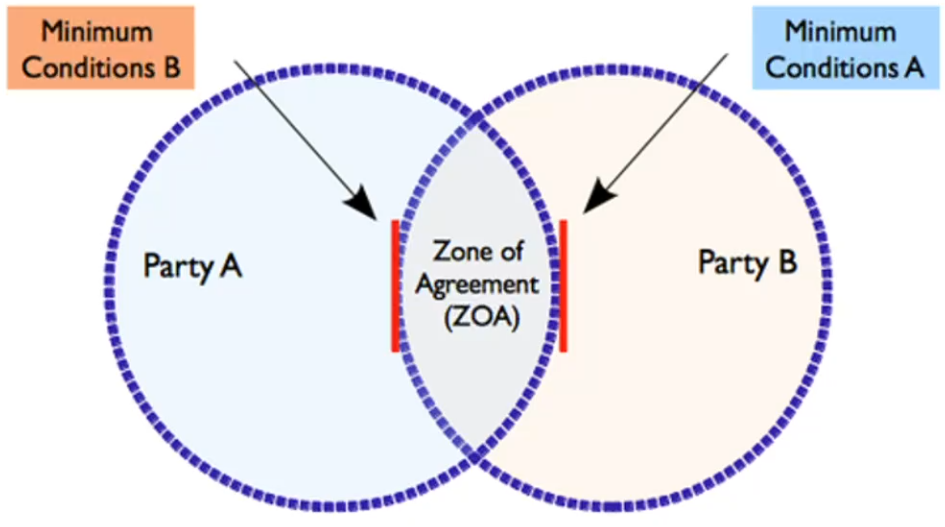
\includegraphics[width=0.4\linewidth]{../images/13-ZOA.png}
				\caption{Zone of agreement}
				\label{fig:13-ZOA}
			\end{figure}
			Due to all the difficulties, a lot of coalitions have formed amongst the smaller delegations which are roughly depicted in figure \ref{fig:13-coalitions}.
			\begin{figure}[h]
				\centering
				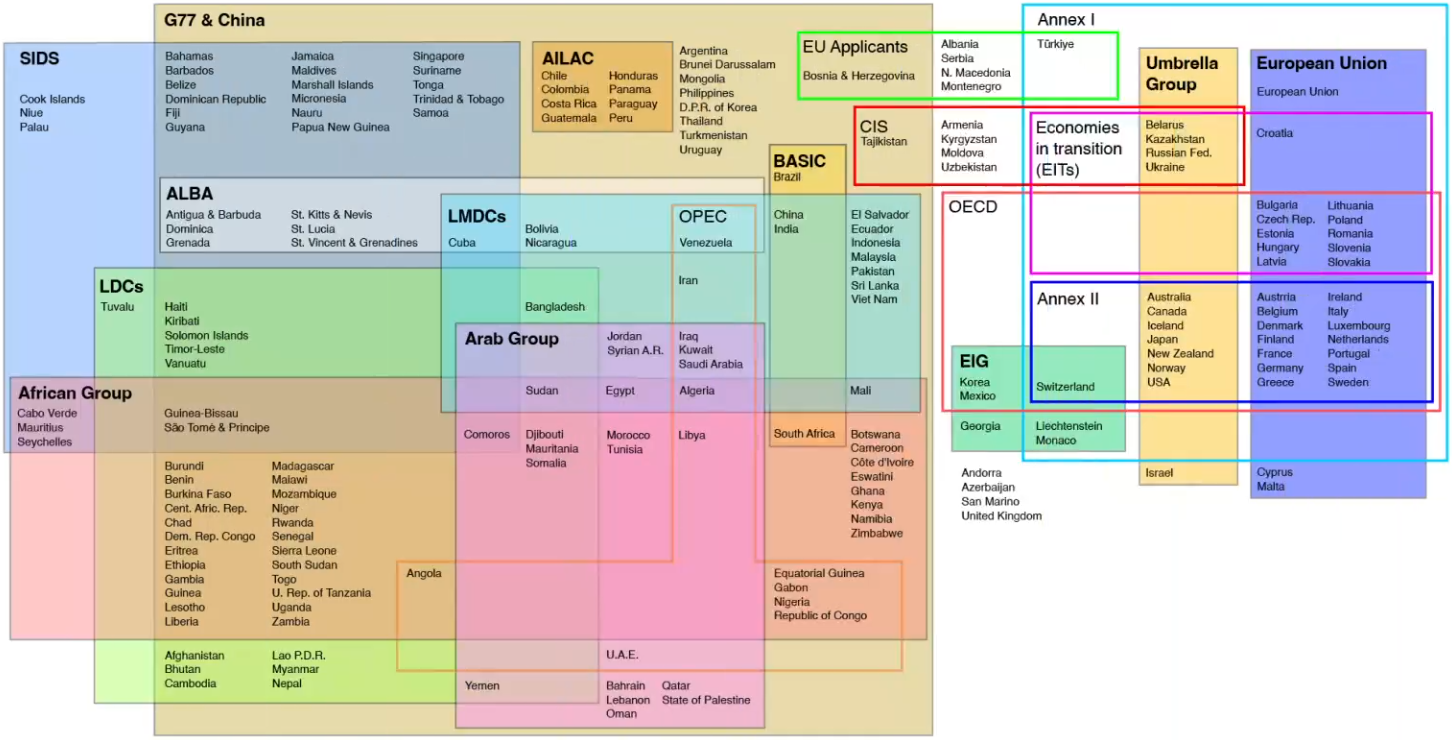
\includegraphics[width=0.7\linewidth]{../images/13-coalitions.png}
				\caption{The coalitions}
				\label{fig:13-coalitions}
			\end{figure}
		
		\subsubsection{Poly-centric governance}
			Poly-centric governance is a complementary perspective to multilateral negotiations. Here, multiple governing authorities adopt their own measures addressing a certain problem. Many environmental problems can be adopted to achieve local benefits in addition to global ones such as solving local air pollution. Each authority adopts measures independently under this system and is not forced to do so. States can still influence each other though by, for example, learning from each other. \\
			\\
			 Is poly-centric governance an effective way to deal with these problems? In some cases, this can certainly be done; but sometimes it is just not possible, so we revert to multilateral negotiations. Usually we fail because of the shortcomings in poly-centric governance:
			 \begin{description}
			 	\item[Leakage] This is when an activity that would occur in one location is simply shifted to another location, the overall problem is thus not solved.
			 	\item[Inconsistent policies] When policies differ, the incentive to develop a technology and innovation may not be high enough given the size of the jurisdiction in which it could be solved. 
			 	\item[Free riding] Some actors can benefit from a policy adopted by others without contributing to addressing the problem.
			 \end{description}

\end{document}